% Harmadik, negyedik és ötödik előadás

\chapter{Adatmanipulációs fa}

\section{Az adatmanipulációs fa fogalma}
Az adatmanipulációs fa megmutatja a potenciális adatmanipulációs lehetőségeket.
Bizonyos részfái megmutatják egy konkrét implementáció adatmanipulációs lehetőségeit.

\section{Részei}
\begin{itemize}
    \item 1. szint: adattípusok, azaz miket értelmezünk az adott architektúrában (pl. 1 byte FX, 2 byte FX, FP, stb.)
    \item 2. szint: műveletek szintje, azaz az adattípusokkal milyen műveletek végezhetők (pl. összeadás, kivonás, logikai műveletek)
    \item 3. szint: operandusok típusai (pl. két operandusos, három operandusos). Megkülönböztetünk memória, regiszter és akkumulátor operandus típusokat.
    \item 4. szint: címzési módok (pl. regiszter+displacement, pc+displacement, index regiszter+displacement, direkt, indirekt)
    \item 5. szint: gépi kód
\end{itemize}

\section{Adattípusok}
Megkülönböztetünk elemi és összetett adattípusokat.
Elsősorban az elemi adattípusokkal foglalkozunk.
Az összetett adattípusok elemiekből épülnek fel, ha különböző típusokból áll össze, akkor rekordnak hívjuk, ha azonos típusokból, akkor megkülönböztetünk vektor (1D tömb), tömb (többdimenziós), szöveg, verem, sor, lista, fa, halmaz adattípusokat.

\subsection{Elemi addattípusok}
Megkülönböztetünk numerikus, karakteres, logikai, pixel és még több adattípust.

\subsubsection{Numerikus adattípusok}
\begin{itemize}
    \item FX
    \item FP
    \item BCD (binárisan kódolt decimális)
    \begin{itemize}
        \item pakolt (1 byte két helyiérték, 4 bit egy decimális szám)
        \item pakolatlan (zónázott)
    \end{itemize}
\end{itemize}

\subsubsection{FX adattípusok}
Kódolás szerint megkülönböztetünk:
\begin{itemize}
    \item egyes komplemens
    \item kettes komplemens
    \begin{itemize}
        \item előjeles (1, 2, 4, 8, 16 byte)
        \item előjel nélküli
    \end{itemize}
    \item többletes kódolás
\end{itemize}

\subsubsection{FP adattípusok}
Megkülönböztetünk:
\begin{itemize}
    \item normalizált
    \begin{itemize}
        \item hexára normalizált
        \item binárisra normalizált
        \begin{itemize}
            \item VAX
            \item IEEE
            \begin{itemize}
                \item 1x pontosságú (32 bites)
                \item 2x pontosságú (64 bites)
                \item kiterjesztett pontosságú (128 bites)
            \end{itemize}
        \end{itemize}
    \end{itemize}
    \item nem normalizált
\end{itemize}
Általában a normalizáltat használják.

\subsubsection{Karakteres adattípusok}
Megkülönböztetünk:
\begin{itemize}
    \item EBDIC (8 bit, 60-as évek)
    \item ASCII
    \begin{itemize}
        \item 7 bites (szabványos)
        \item 8 bites (kiterjesztett)
    \end{itemize}
    \item Unicode (2 byte)
\end{itemize}

\subsubsection{Logikai adattípusok}
Megkülönböztetünk:
\begin{itemize}
    \item 1 byte
    \item 2 byte
    \item 4 byte
    \item változó hosszú
\end{itemize}
Példák: AND, OR eredményei.
Általában 1 bit értékes (általában a legmagasabb helyiérték).

\section{Műveletek}
Az adatmanipulációs fa minden művelet esetén megállapítja, hogy milyen utasítás típusok vannak megengedve és milyen operandus típus választható.
Az utasítás a számítógép által végrehajtható alapvető feladatok ellátására szolgáló elemi művelet leírása.

\subsection{Utasítás végrehajtás menete}
Egy gépi kódú utasítás általában két részből áll: MK, azaz műveleti kód és címrész.
Az MK tartalmazza, hogy mit kell csinálni, a címrész pedig, hogy melyik címen lévő adattal.
Pl.: ADD r3,r1,r2.
Általánosan az utasítás végrehajtás lépései:
\begin{enumerate}
    \item A processzor megnézi, hogy van-e megszakítás kérés, ha van, kiszolgálja azt
    \item Ha nem történt megszakítás kérés, lehívja az utasítást
    \item Végrehajtja az utasítást
\end{enumerate}

A processzor főbb regiszterei láthatók a következő ábrán.
\begin{figure}[H]
    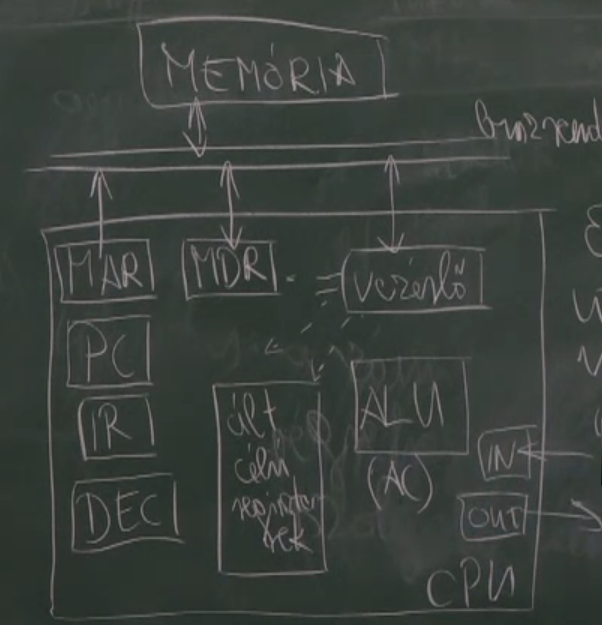
\includegraphics[width=0.8\textwidth]{regs}
    \centering
    \caption{Egy CPU főbb regiszterei}
    \label{fig:regs}
\end{figure}

Egy gépi kódú utasítás elemi műveletek sorozataként írható fel.
Példa: ADD r1, r2 utasítás végrehajtása:
\begin{enumerate}
    \item FETCH - az utasítást le kell hívni:
    \begin{enumerate}
        \item A processzor a program counter (PC) értékét betölti a memória címregiszterbe (MAR).
        \item A címregiszterben lévő címen lévő értéket betölti a memória adatregiszterbe (MDR).
        \item A memória adatregiszter tartalmát áttölti az utasításregiszterbe (IR)
        \item A program counter értékét egy egységgel inkrementálja
    \end{enumerate}
    \item Dekódolás és operandus betöltés
    \begin{enumerate}
        \item Az utasításregiszter tartalmát betölti a processzor a dekóderbe (DEC)
        \item Az utasítás címrész tartalmát betölti a memória címregiszterbe
        \item A memória címregiszter értékének címén található adatot betölti a memória adatregiszterbe
        \item A memória adatregiszter tartalmát betölti az akkumulátorba
    \end{enumerate}
    \item Művelet végrehajtás
    \begin{enumerate}
        \item A dekóder megfelelő (másik) címrésze bekerül a MAR-ba
        \item A MAR értékének címén lévő adat bekerül az MDR-be
        \item Az AC-be betölti az AC+MDR-t (elvégzi az összeadást)
    \end{enumerate}
    \item Az eremény tárolása (STORE)
    \begin{enumerate}
        \item A dekóder címrésze (ugyanaz mint a dekódolásnál) bekerül a memória címregiszterbe
        \item Az akkumulátor tartalmát áttölti az MDR-be
        \item Az MDR tartalmát betölti az MAR által mutatott címre
    \end{enumerate}
\end{enumerate}

Példa: JMP utasítás
\begin{enumerate}
    \item IR-ből betölti a dekóderbe az utasítást
    \item A dekóder címrészét betölti MAR-ba
    \item A MAR által mutatott értékkel felülírja PC-t
\end{enumerate}

\subsection{Utasítások részei}
\begin{itemize}
    \item műveleti kód
    \item operandus
    \begin{itemize}
        \item cél (dest op)
        \item forrás (source op)
    \end{itemize}
\end{itemize}

\subsection{Utasítások típusai címek száma alapján}
\begin{itemize}
    \item 4 címes: cél, forrás 1, forrás 2, következő utasítás címe. Hátránya, hogy nehézkes és merev.
    \item 3 címes: cél, forrás 1, forrás 2. A következő utasítás címét helyettesítették az auto inkrementálódó PC-vel. RISC architektúrák használják. Előnye a szabadság és a párhuzamosítási lehetőség, hátránya, hogy bonyolultabbak és hosszabbak az utasítások.
    \item 2 címes: nincs cél operandus, csak forrás 1 és 2. Az eredmény felülírja a forrás 1-et. CISC processzorok használják (pl. x86). Előnye az egyszerűbb utasítás, hátránya, hogy felülírja az egyik forrás operandust.
    \item 1 címes: be kell tölteni az egyik operandust az akkumulátorba, majd a második operandussal módosítjuk AC tartalmát. Pl. ADD utasítás: LOAD[100], ADD[101]. Hátránya, hogy az utasítások száma nő, viszont az utasítások kisebbek és gyorsabban végrehajthatóak. Többszörös összeadásnál hasznos például.
    \item 0 címes: pl. NOP, CLEAR D (flag), PUSH, POP. A stack utasítások gyorsaságát is ez adja, nem kell külön megcímezni, hanem a stack pointer értékét használja. Előnye, hogy gyors, hátránya, hogy növelik az utasításkészletet.
\end{itemize}

A három címes utasítások mindhárom operandusa regiszter típusú, a két címeseknél viszont általában a második operandus lehet memória típusú is.

\section{Operandus típusok}
\begin{itemize}
    \item AC - akkumulátor: gyors, de csak egy van belőle
    \item memória: nagy, hosszú címe van és viszonylag lassú
    \item regiszter: gyors, de korlátozott számú
    \item verem: nagyon gyors, de csak a tetejét látjuk, így sok adatot nem lehet benne tárolni
    \item immediate: nem egy címet adunk meg, hanem közvetlenül a programba írjuk be az operandus értékét. Nagyon gyors, de a módosításához módosítani kell a programot.
\end{itemize}

\subsection{Architektúrák osztályozása operandus típusok szerint}
\begin{itemize}
    \item szabályos: csak egy fajta operandus típus engedélyezett (kivéve akkumulátor, mert abból csak egy van)
    \begin{itemize}
        \item akkumulátor (akkumulátor-regiszter és akkumulátor-memória)
        \item memória (memória-memória, memória-memória-memória)
        \item regiszter (regiszter-regiszter, regiszter-regiszter-regiszter)
        \item stack (stack-stack, stack-stack-stack)
    \end{itemize}
    \item kombinált: a különböző operandus típusok megengedettek egy utasításon belül (pl. regiszter + memória) - nem homogén.
\end{itemize}

A szabályos architektúrák kezelése és tervezése könnyebb.
Ilyenek pl. a RISC architektúrák (mint pl. ARM), amik 3 címes regiszter típusú operandusokkal dolgoznak.
A memória eléréséhez két kivételes utasítás használható: LOAD és STORE.

Kombinált architektúra pl. a CISC architektúrák (mint pl. x86).

\section{Címzési módok}
A címzési mód maga a címszámítási algoritmus.
Ezt 3, egymástól független elem kombinációja adja:
\begin{itemize}
    \item címszámítás: jelzi, hogy abszolút, vagy relatív címzést használunk. Az abszolút címzés a teljes címet tartalmazza, a relatívnál pedig egy bázishoz képest számoljuk. A relatív gyorsabb, rövidebbek a címek, de deklarálni kell a bázis címet és a címszámítási algoritmust. Elsősorban a relatív címzés van használatban.
    \item cím módosítás (opcionális komponens): indexelés, auto inkrementálás, auto dekrementálás. Segítségével könnyebben meghatározható a következő operandus címe.
    \item deklarált (tényleges) cím meghatározása: azt jelenti, hogy a címet direkt vagy indirekt, illetve valós vagy virtuális címként interpretáljuk.
\end{itemize}

\subsection{Relatív címszámítás}
A CPU címtere nagyon nagy (4-64 TB), így abszolút címzéssel nagyon nagy címeket kéne kezelni.
Ezért inkább a relatív címzést használják.
Bázis címnek választható pl. a PC, a stack teteje, valamilyen index regiszter, stb.

\subsection{Az indexelés és az index regiszter}
Megkülönböztetünk egyedi és blokkos címzést, jellemzően blokkokat címzünk és töltünk be a gyorsítótárba.
Ehhez szükség van egy index regiszterre, amiben az eltolás tárolódik.
Több dimenziós blokkoknál több index regiszter van használatban.

\section{Utasítás kód}
Az adatmanipulációs fa legalsó szintje, gépi reprezentációnként különböző.

\section{Állapottér}
Az állapottér olyan, programból látható és nem látható (program transzparens) tárolókból áll, amelyek az adott programra vonatkozó állapotinformációkat hordozzák.
A program transzparens információk a rendszerfunkciókhoz szükségesek, mint pl. virtuális memória kezelés és a megszakításkezelés.
Az állapottér tehát felosztható:
\begin{itemize}
    \item transzparens
    \begin{itemize}
        \item virtuális memória kezelés
        \item megszakításkezelés
        \item veremkezelés
    \end{itemize}
    \item látható
    \begin{itemize}
        \item PC
        \item státusz indikátorok (flagek)
        \begin{itemize}
            \item CC (Condition Code, IBM gépeknél): két bit, különböző állapotinfókat tartalmaz
            \item univerzális állapotjelzők pl. carry, zero
            \item adattípusonként különböző állapotjelzők pl. denormalizált szám vagy érvénytelen művelet (minden regiszterkészlethez definiáltak)
        \end{itemize}
        \item indexelés
        \item címzési módok
        \item debug
    \end{itemize}
\end{itemize}

\subsection{Flagek}
Olyan kivételes események figyelésére és vezérlésére szolgálnak, melyek a program futása közben általánosságban jelenhetnek meg.
Ilyen pl. a túlcsordulás vagy a nullával való osztás.

\subsection{Állapot műveletek}
Az állapotjelzőket speciális utasításokkal lehet manipulálni.
Állapotműveletek PC esetén:
\begin{itemize}
    \item inkrementálás
    \item dekrementálás
    \item felülírás (pl. egy utasításból vett címmel, ugróutasítással)
\end{itemize}
Flagek esetén:
\begin{itemize}
    \item mentés
    \item beállítás
    \item reset
    \item load
    \item clear
\end{itemize}